\chapter{Experiments and results}

We evaluate our software for isometric reconciliation on a simulated and real dataset that were used to evaluate SPIMAP \cite{spimap} and TreeFix \cite{treefix} in previous studies. The simulated dataset consists of 1000 simulated gene families of two clades of species: 12 \emph{Drosophila} genomes and 16 fungal genomes, generated with the SPIMAP model. The real dataset includes 5351 real gene families from 16 fungal genomes.

To compare the results, we run other software for computing the gene tree reconciliation: Notung \cite{notung}, TreeFix \cite{treefix} and Treerecs \cite{treerecs}, on the same dataset.

\section{Simulated dataset}

In the simulated dataset, we know the correct gene tree with its evolutionary events, which allows us to test several aspects. We evaluate our software for isometric reconciliation for two cases: without rerooting the gene tree and with rerooting the gene tree. In the experiments, we measure the precision of inferred duplications and gene losses, the average runtime for computing the results for each gene tree and the number of gene trees without solution, as our isometric reconciliation software takes branch lengths into account and occasionally the gene tree can not fit the species tree correctly, because some small errors in branch lengths. In the second case with rerooting the gene tree, we also measure the precision of the correctly inferred root.

\subsection{Without rerooting the gene tree} \label{without_rerooting_the_gene_tree}

We take the rooted gene tree as it is from the dataset and run a reconciliation with \emph{countDL} function (Algorithm \ref{countDL} in Chapter \ref{main_algorithm}). We evaluate it several times with different tolerance setting to scale up the edges. The tolerance setting are $0.0, \num{1e-6}, \num{1e-5}, \num{1e-3}, 0.1, 0.3, 0.5, 1.0$ and the $\epsilon = \num{1e-6}$. We compare our results with only Notung and Treerecs, as the TreeFix software automatically reroot the given gene tree.

\noindent\textbf{Flies dataset}

On the flies dataset (Tab. \ref{flies_without_rerooting}), our software has a problem to infer reconciliation for all gene trees with tolerance set to $0.0$, thus $3.97\%$ of the gene trees are without reconciliation. Still, the reconciled trees have perfect precision and sensitivity of inferred duplication and gene losses. With the tolerance set to $\num{1e-6}$, we computed isometric reconciliation for all gene trees, but some nodes are incorrectly detected as duplications or gene losses, so the inferred duplications have precision $99.93\%$ with the sensitivity of $100\%$ and gene losses has precision $99.76\%$ with the sensitivity of $99.98\%$. It is caused by a rounding error on the last decimal place since the edge length of the gene trees in the dataset has 6 decimal places. Higher tolerance settings show the same results, where our isometric reconciliation software infer reconciliation for all gene trees from the dataset with $100\%$ precision and sensitivity of duplication and gene losses. The Notung and Treerecs computed reconciliation for all gene trees with perfect precision and sensitivity of inferred duplication and gene losses. However, the average running time for each gene tree is best in our reconciliation software, which is about $0.003617$ for each tree in each tolerance setting. In comparison, the Treerecs average time is bigger by $90.23\%$ from our average running time. The Notung has the longest average time, which is bigger by $94.49\%$ from the Treerecs average running time and by $99.46\%$ from our average running time.

\begin{table}[ht!]
\caption{Flies: results of phylogenetic software on simulated dataset without rerooting the gene tree}
\centering
\begin{threeparttable}
\begin{tabular}{| m{0.25\textwidth} | >{\centering\arraybackslash}m{0.115\textwidth} | >{\centering\arraybackslash}m{0.08\textwidth} | >{\centering\arraybackslash}m{0.08\textwidth} | >{\centering\arraybackslash}m{0.08\textwidth} | >{\centering\arraybackslash}m{0.08\textwidth} | >{\centering\arraybackslash}m{0.115\textwidth} |}
   \hline
     \multirow{2}{*}{\textbf{Software\textsuperscript{a}}} &
     \multirow{2}{*}{\textbf{W/o sol\textsuperscript{b}}} & 
     \multicolumn{2}{c|}{\textbf{Duplication}} &
     \multicolumn{2}{c|}{\textbf{Gene loss}} &
     \multirow{2}{*}{\textbf{Runtime\textsuperscript{g}}}\\
     \cline{3-6}
     & & \textbf{Prec\textsuperscript{c}} & \textbf{Sens\textsuperscript{d}} & \textbf{Prec\textsuperscript{e}} & \textbf{Sens\textsuperscript{f}} & \\
    \hline
    Our (t - 0.0) & 3.97 & 100 & 100 & 100 & 100 & 0.007415\\
    Our (t - \num{1e-6}) & 0 & 99.93 & 100 & 99.76 & 99.98 & 0.008160\\
    Our (t - \num{1e-5}) & 0 & 100 & 100 & 100 & 100 & 0.003050\\
    Our (t - \num{1e-3}) & 0 & 100 & 100 & 100 & 100 & 0.003026\\
    Our (t - 0.1) & 0 & 100 & 100 & 100 & 100 & 0.001785\\
    Our (t - 0.3) & 0 & 100 & 100 & 100 & 100 & 0.001771\\
    Our (t - 0.5) & 0 & 100 & 100 & 100 & 100 & 0.001919\\
    Our (t - 1.0) & 0 & 100 & 100 & 100 & 100 & 0.001810\\
    Notung  & 0 & 100 & 100 & 100 & 100 & 0.671599\\
    Treerecs  & 0 & 100 & 100 & 100 & 100 & 0.037014\\
    \hline
  \end{tabular}
  \begin{tablenotes}
                 \footnotesize
                 \item[a] Phylogenetic software with \emph{"t"} as tolerance setting.
                 \item[b] Percentage of gene trees without a solution.
                 \item[c] Precision of inferred duplications.
                 \item[d] Sensitivity of inferred duplications.
                 \item[e] Precision of inferred gene losses.
                 \item[f] Sensitivity of inferred gene losses.
                 \item[g] Average runtime of computing the reconciliation for each gene tree in seconds.
             \end{tablenotes}
         \end{threeparttable}
  \label{flies_without_rerooting}
\end{table}

\noindent \textbf{Fungi dataset}

The results for the fungi dataset (Tab. \ref{fungi_without_rerooting}) are similar to the results for the flies dataset. Our isometric reconciliation software has also a problem inferring reconciliation for all gene trees with a tolerance setting of $0.0$, ergo the $9.03\%$ of gene trees has no reconciliation solution. For the remaining $90.97\%$ of gene trees, our software finds the correct reconciliation with $100\%$ precision and sensitivity of inferred duplications and gene losses. Our software recognizes isometric reconciliation for all gene trees from the dataset with tolerance set to \num{1e-6}, but the precision of duplications and gene losses decrease to $99.99\%$ and $99.98\%$, respectively, because of the rounding error on the last decimal place since the edge lengths of gene trees from the fungi dataset has also 6 decimal places. However, the sensitivity of inferred duplications and gene losses stays $100\%$. With the remaining tolerance setting, we infer reconciliation for all gene trees from the dataset with perfect precision and sensitivity of duplications and gene losses. The other software, Notung and Treerecs, compute reconciliation for all gene trees with $100\%$ precision and sensitivity of inferred duplications and gene losses. To compare the average running time for each gene tree, our software has the best average running time about $0.004006$ for each tolerance setting. The Treerecs has the second-best average running time bigger by $93.11\%$ from our average running time. The longest average running time has Notung, which is bigger by $91.8\%$ from the Treerecs average running time and by $99.43\%$ from our average running time.

\begin{table}[ht!]
\caption{Fungi: results of phylogenetic software on simulated dataset without rerooting the gene tree}
\centering
 \begin{threeparttable}
\begin{tabular}{| m{0.25\textwidth} | >{\centering\arraybackslash}m{0.115\textwidth} | >{\centering\arraybackslash}m{0.08\textwidth} | >{\centering\arraybackslash}m{0.08\textwidth} | >{\centering\arraybackslash}m{0.08\textwidth} | >{\centering\arraybackslash}m{0.08\textwidth} | >{\centering\arraybackslash}m{0.115\textwidth} |}
   \hline
     \multirow{2}{*}{\textbf{Software\textsuperscript{a}}} &
     \multirow{2}{*}{\textbf{W/o sol\textsuperscript{b}}} & 
     \multicolumn{2}{c|}{\textbf{Duplication}} &
     \multicolumn{2}{c|}{\textbf{Gene loss}} &
     \multirow{2}{*}{\textbf{Runtime\textsuperscript{g}}}\\
     \cline{3-6}
     & & \textbf{Prec\textsuperscript{c}} & \textbf{Sens\textsuperscript{d}} & \textbf{Prec\textsuperscript{e}} & \textbf{Sens\textsuperscript{f}} & \\
    \hline
    Our (t - 0.0) & 9.03 & 100 & 100 & 100 & 100 & 0.007225\\
    Our (t - \num{1e-6}) & 0 & 99.99 & 100 & 99.98 & 100 & 0.005962\\
    Our (t - \num{1e-5}) & 0 & 100 & 100 & 100 & 100 & 0.003898\\
    Our (t - \num{1e-3}) & 0 & 100 & 100 & 100 & 100 & 0.004728\\
    Our (t - 0.1) & 0 & 100 & 100 & 100 & 100 & 0.003158\\
    Our (t - 0.3) & 0 & 100 & 100 & 100 & 100 & 0.002231\\
    Our (t - 0.5) & 0 & 100 & 100 & 100 & 100 & 0.002366\\
    Our (t - 1.0) & 0 & 100 & 100 & 100 & 100 & 0.002481\\
    Notung  & 0 & 100 & 100 & 100 & 100 & 0.708665\\
    Treerecs  & 0 & 100 & 100 & 100 & 100 & 0.058145\\
    \hline
  \end{tabular}
    \begin{tablenotes}
                \footnotesize
                 \item[a] Phylogenetic software with \emph{"t"} as tolerance setting.
                 \item[b] Percentage of gene trees without a solution.
                 \item[c] Precision of inferred duplications.
                 \item[d] Sensitivity of inferred duplications.
                 \item[e] Precision of inferred gene losses.
                 \item[f] Sensitivity of inferred gene losses.
                 \item[g] Average runtime of computing the reconciliation for each gene tree in seconds.
             \end{tablenotes}
         \end{threeparttable}
  \label{fungi_without_rerooting}
\end{table}

\noindent \textbf{Conclusion}

To sum up, our software runs the best with tolerance \num {1e-5}, which is by one decimal place shorter than the edge length of gene trees from both datasets. Thus, if the tolerance has less than or an equal number of decimal places, our software may not find reconciliation for all rooted gene trees or may find a reconciliation with wrongly detected duplications and gene losses, which decreases the precision and sensitivity of inferred duplications and gene losses. In terms of time, our software infers the reconciliation for each gene tree the fastest compared to the Notung and Treerecs.


\subsection{With rerooting the gene tree}

The software for isometric reconciliation takes the rooted gene tree as input with an argument to reroot the given gene tree. We forget the root of the rooted gene tree and transform it into the unrooted gene tree. On the obtained unrooted gene tree, we run the \emph{getIntervals} function (Algorithm \ref{getIntervals} in Chapter \ref{rooting_the_gene_tree}) to get a set of roots given by a pair of intervals for subdividing each edge of the unrooted gene tree, where the first interval from the pair signifies the edge length on the left from the new root and the second interval from the pair signifies the edge length on the right from the new root. Then we run a reconciliation with \emph{countDL} function (Algorithm \ref{countDL} in Chapter \ref{main_algorithm}). We want to find a new root minimizing the number of inferred duplications and gene losses in reconciliation. The process is executed several times with different tolerance and step settings. The tolerance and $\epsilon$ setting are the same as in the first case without rerooting the gene tree (Chapter \ref{without_rerooting_the_gene_tree}). The step settings are $0.0, 0.1, 0.3, 0.5, 1.0, 2.0$ since the edge lengths of species trees and gene trees from the dataset are in a range from about $1$ to $78$ expressed in million years.

\noindent \textbf{Flies dataset}

At first, we run our software with all tolerance settings and step set to $0.0$, as we can see in Table \ref{flies_with_rerooting}, where for each edge $(u, v) \in E(G)$, the \emph{getIntervals} function returns a set of roots subdividing the edge right above the vertices $u$ and $v$. Because of that, our software is not able to infer reconciliation for all gene trees at all tolerance settings. It not finds any reconciliation with tolerance set to $0.0, \num{1e-6}, \num{1e-5}, \num{1e-3}$. With the tolerance of $0.1$, it recognizes the first isometric reconciliations for $82.37\%$ of gene trees from the dataset. The percentage of gene trees without computed reconciliation decreases with the increasing tolerance. With the tolerance of $1.0$, only $0.48\%$ of gene trees does not have inferred reconciliation. As our software does not find solutions for the reconciliation with the first 4 tolerance settings, we can not calculate and compare the precision of inferred root and precision and sensitivity of inferred duplications or gene losses. For the remaining tolerance settings, the precision of correctly inferred root is highest with tolerance set to $1.0$. It rises with increasing tolerance. A slight decrease is between tolerances $0.3$ and $0.5$ caused by newly inferred reconciliations for gene trees that have no solution with tolerance $0.3$ but find a solution with tolerance $0.5$. The precision of inferred duplications has a growing tendency for all remaining tolerance settings. The sensitivity of inferred duplications is sensitive to the rooting of a gene tree on a different edge than the original edge, so when the precision of correctly inferred root drops between tolerances $0.3$ and $0.5$, the sensitivity drops by $0.09\%$ too. Finding the root on different edge induces duplications and gene losses on different nodes. Apart from that, it has an increasing tendency. The precision of inferred gene losses is increasing for the remaining tolerance settings with a slight drop of $0.01\%$ between tolerances $0.3$ and $0.5$ also caused by the wrongly inferred roots. The sensitivity of inferred gene losses is highest with the tolerance of $0.1$ and then it drops by $18.56\%$. It is induced by a decrease in the percentage of gene trees without solutions, where we infer reconciliation for more gene trees with tolerance $0.3$ than with the tolerance $0.1$, but some of them has wrongly inferred gene losses, where the gene loss is not supposed to be. Besides this drop, it has a growing tendency from tolerance $0.3$ to tolerance $1.0$.

With step set to $0.1$, we find reconciliation solutions already at tolerance set to $0.0$ for $1.65\%$ gene trees from the dataset. The percentage of gene trees without solution decreases as the tolerance increase and it is $0\%$ from tolerance $0.1$ and more. The precision of correctly inferred root is $100\%$ for tolerance settings from $0.0$ till $0.1$ include. It does not even drop with the big increase of inferred reconciliations between tolerances \num{1e-5} and \num{1e-3} for gene trees that have not solution at tolerance \num{1e-5}, but the solution exists at tolerance \num{1e-3}. It starts decreasing with tolerance $0.3$ and bigger induced by increasing tolerance, allowing finding a solution on another edge than the original edge with a better reconciliation score. The precision of inferred duplications has similar development as the precision of correctly inferred root with one exception at the tolerance set to \num{1e-3}. The high increase of gene trees with solution caused a big drop, where a lot of these solution contains wrongly inferred duplications which correct the increase in tolerance to $0.1$. The decrease from tolerance set to $0.3$ and more is caused by a change in finding a different root, which induces duplications on different nodes. The sensitivity of inferred duplications is perfect for tolerances from $0.0$ to $0.1$ include. It starts decreasing between tolerances $0.1$ and $0.3$ induced for the same reason as the decrease in precision of inferred duplications. The precision of inferred gene losses is perfect except tolerance set to \num{1e-3}, where the cause of the drop is the same as for the precision of inferred duplications. The sensitivity of inferred gene losses is perfect until it starts decreasing between tolerances $0.1$ and $0.3$ caused by finding a reconciliation solution with different root and fewer gene losses, where the inferred gene losses are correct, as shown by the precision of inferred gene losses, but we do not find all expected gene losses.

The next tested step setting is $0.3$, where the results are almost the same as the result with the step setting $0.1$ with the exception for tolerances set to \num{1e-3} and $0.1$. At the tolerance \num{1e-3}, we are not able to infer solutions for as many gene trees as with step set to $0.1$. Still, the $4.27\%$ increase in inferred reconciliation solutions for gene trees between tolerances \num{1e-5} and \num{1e-3} induces a decrease in precision of inferred duplications and gene losses. The second exception is at the tolerance $0.1$, where the precision of inferred duplications and gene losses are $99.89\%$ and $99.72\%$, respectively, again caused by a big increase of inferred solutions for gene trees with no solution at tolerance \num{1e-3} and a found solution at tolerance $0.1$, where some of these solutions have incorrectly detected duplications and gene losses.

\begin{table}[!htbp]
\caption{Flies: results of phylogenetic software on simulated dataset with rerooting the gene tree}
\footnotesize
\centering
 \begin{threeparttable}
  \begin{tabular}{| m{0.25\textwidth} | >{\centering\arraybackslash}m{0.1\textwidth} | >{\centering\arraybackslash}m{0.06\textwidth} | >{\centering\arraybackslash}m{0.06\textwidth} | >{\centering\arraybackslash}m{0.06\textwidth} | >{\centering\arraybackslash}m{0.06\textwidth} | >{\centering\arraybackslash}m{0.06\textwidth} | >{\centering\arraybackslash}m{0.1\textwidth} |}
  \hline
      \multirow{2}{*}{\textbf{Software\textsuperscript{a}}} &
     \multirow{2}{*}{\textbf{W/o sol\textsuperscript{b}}} & 
     \multirow{2}{*}{\textbf{Root\textsuperscript{c}}} &
     \multicolumn{2}{c|}{\textbf{Duplication\textsuperscript{d}}} &
     \multicolumn{2}{c|}{\textbf{Gene loss\textsuperscript{e}}} &
     \multirow{2}{*}{\textbf{Runtime\textsuperscript{f}}}\\
     \cline{4-7}
     & & & \textbf{Prec} & \textbf{Sens} & \textbf{Prec} & \textbf{Sens} & \\
    \hline
    Our (t - 0.0; s - 0.0) & 100 & - & - & - & - & - & 0.004377\\
    Our (t - \num{1e-6}; s - 0.0) & 100 & - & - & - & - & - & 0.002373\\
    Our (t - \num{1e-5}; s - 0.0) & 100 & - & - & - & - & - & 0.002402\\
    Our (t - \num{1e-3}; s - 0.0) & 100 & - & - & - & - & - & 0.002352\\
    Our (t - 0.1; s - 0.0) & 17.63 & 98.64 & 25.42 & 98.58 & 8.99 & 99.42 & 0.004743\\
    Our (t - 0.3; s - 0.0) & 2.47 & 99.47 & 45.56 & 99.44 & 17.61 & 80.86 & 0.005165\\
    Our (t - 0.5; s - 0.0) & 2.32 & 99.39 & 45.63 & 99.35 & 17.60 & 80.99 & 0.005745\\
    Our (t - 1.0; s - 0.0) & 0.48 & 99.98 & 46.37 & 99.98 & 23.23 & 91.98 & 0.005148\\
    \hline
    Our (t - 0.0; s - 0.1) & 98.35 & 100 & 100 & 100 & 100 & 100 & 0.213234\\
    Our (t - \num{1e-6}; s - 0.1) & 98.3 & 100 & 100 & 100 & 100 & 100 & 0.315081\\
    Our (t - \num{1e-5}; s - 0.1) & 98.3 & 100 & 100 & 100 & 100 & 100 & 0.237645\\
    Our (t - \num{1e-3}; s - 0.1) & 0.28 & 100 & 34.6 & 100 & 17.03 & 100 & 0.460089\\
    Our (t - 0.1; s - 0.1) & 0 & 100 & 100 & 100 & 100 & 100 & 0.500895\\
    Our (t - 0.3; s - 0.1) & 0 & 99.93 & 99.95 & 99.95 & 100 & 99.94 & 0.622866\\
    Our (t - 0.5; s - 0.1) & 0 & 99.81 & 99.86 & 99.86 & 100 & 99.83 & 0.777619\\
    Our (t - 1.0; s - 0.1) & 0 & 99.65 & 99.76 & 99.76 & 100 & 99.70 & 0.914920\\
    \hline
    Our (t - 0.0; s - 0.3) & 98.35 & 100 & 100 & 100 & 100 & 100 & 0.042934\\
    Our (t - \num{1e-6}; s - 0.3) & 98.3 & 100 & 100 & 100 & 100 & 100 & 0.046455\\
    Our (t - \num{1e-5}; s - 0.3) & 98.3 & 100 & 100 & 100 & 100 & 100 & 0.047223\\
    Our (t - \num{1e-3}; s - 0.3) & 94.03 & 100 & 25.77 & 100 & 17.15 & 100 & 0.047767\\
    Our (t - 0.1; s - 0.3) & 0 & 100 & 99.91 & 100 & 99.76 & 100 & 0.100275\\
    Our (t - 0.3; s - 0.3) & 0 & 99.96 & 99.96 & 99.96 & 100 & 99.95 & 0.121550\\
    Our (t - 0.5; s - 0.3) & 0 & 99.89 & 99.91 & 99.91 & 100 & 99.88 & 0.144801\\
    Our (t - 1.0; s - 0.3) & 0 & 99.77 & 99.82 & 99.82 & 100 & 99.77 & 0.172164\\
    \hline
    Our (t - 0.0; s - 0.5) & 100 & - & - & - & - & - & 0.027602\\
    Our (t - \num{1e-6}; s - 0.5) & 100 & - & - & - & - & - & 0.027832\\
    Our (t - \num{1e-5}; s - 0.5) & 100 & - & - & - & - & - & 0.028455\\
    Our (t - \num{1e-3}; s - 0.5) & 18.03 & 100 & 31.96 & 100 & 12.33 & 100 & 0.052290\\
    Our (t - 0.1; s - 0.5) & 0 & 100 & 100 & 100 & 100 & 100 & 0.059033\\
    Our (t - 0.3; s - 0.5) & 0 & 99.96 & 99.96 & 99.96 & 100 & 99.95 & 0.072567\\
    Our (t - 0.5; s - 0.5) & 0 & 99.92 & 99.93 & 99.93 & 100 & 99.91 & 0.088120\\
    Our (t - 1.0; s - 0.5) & 0 & 99.83 & 99.86 & 99.86 & 100 & 99.81 & 0.109294\\
    \hline
    Our (t - 0.0; s - 1.0) & 100 & - & - & - & - & - & 0.014088\\
    Our (t - \num{1e-6}; s - 1.0) & 100 & - & - & - & - & - & 0.017554\\
    Our (t - \num{1e-5}; s - 1.0) & 100 & - & - & - & - & - & 0.015989\\
    Our (t - \num{1e-3}; s - 1.0) & 18.32 & 100 & 31.91 & 100 & 12.26 & 100 & 0.028652\\
    Our (t - 0.1; s - 1.0) & 0 & 100 & 99.77 & 100 & 99.42 & 100 & 0.031903\\
    Our (t - 0.3; s - 1.0) & 0 & 99.97 & 99.95 & 99.97 & 99.96 & 99.96 & 0.038490\\
    Our (t - 0.5; s - 1.0) & 0 & 99.94 & 99.94 & 99.94 & 100 & 99.92 & 0.045830\\
    Our (t - 1.0; s - 1.0) & 0 & 99.89 & 99.90 & 99.90 & 100 & 99.87 & 0.053317\\
    \hline
    Our (t - 0.0; s - 2.0) & 100 & - & - & - & - & - & 0.008342\\
    Our (t - \num{1e-6}; s - 2.0) & 100 & - & - & - & - & - & 0.009238\\
    Our (t - \num{1e-5}; s - 2.0) & 100 & - & - & - & - & - & 0.009383\\
    Our (t - \num{1e-3}; s - 2.0) & 99.97 & 100 & 50 & 100 & 60 & 100 & 0.009198\\
    Our (t - 0.1; s - 2.0) & 0 & 99.29 & 94.95 & 99.26 & 87.47 & 100 & 0.018753\\
    Our (t - 0.3; s - 2.0) & 0 & 99.87 & 99.17 & 99.87 & 98.02 & 99.96 & 0.022397\\
    Our (t - 0.5; s - 2.0) & 0 & 99.95 & 99.95 & 99.95 & 100 & 99.94 & 0.025403\\
    Our (t - 1.0; s - 2.0) & 0 & 99.93 & 99.93 & 99.93 & 100 & 99.91 & 0.028850\\
    \hline
    Notung & 0 & 92.63 & 99.98 & 99.98 & 93.32 & 93.3 & 1.689122\\
    Treerecs & 0 & 81.07 & 99.09 & 99.09 & 96.12 & 95.14 & 0.081646\\
    TreeFix & 0 & 99.98 & 98.98 & 98.94 & 100 & 98.68 & 4.065790\\
    \hline
  \end{tabular}
   \begin{tablenotes}
                 \scriptsize
                 \item[a] Phylogenetic software with \emph{"t"} as tolerance setting and \emph{"s"} as step setting.
                 \item[b] Percentage of gene trees without a solution.
                 \item[c] Precision of correctly inferred root.
                 \item[d] Precision (\emph{"Prec"}) and sensitivity (\emph{"Sens"}) of inferred duplications.
                 \item[e] Precision (\emph{"Prec"}) and sensitivity (\emph{"Sens"}) of inferred gene losses.
                 \item[f] Average runtime of computing the reconciliation for each gene tree in seconds.
             \end{tablenotes}
         \end{threeparttable}
  \label{flies_with_rerooting}
\end{table}

The step set to $0.5$ is big enough that our software is not capable to find a solution for gene trees with tolerance from $0.0$ till \num{1e-5} include. It finds solutions for $81.97\%$ of the gene trees from the dataset at tolerance \num{1e-3}. For the tolerance $0.1$ and more, the percentage of gene trees without a solution is $0\%$. The precision of correctly inferred root is best at tolerances set to \num{1e-3} and $0.1$ as in the step setting before. It begins decreasing with tolerance $0.3$ and more, where it finds solutions with better reconciliation score while rooting the gene trees at other edges. The precision of inferred duplications is low at tolerance \num{1e-3}, where the gene trees are not able to fit right into the species tree and create more duplications and gene losses than are correct. The precision of inferred duplications decreases with increasing tolerance as the software finds different root and also different duplications on different nodes. The sensitivity of inferred duplications is perfect until tolerance set to $0.3$ and more, where our software finds a root on a different edge than expected causing us not to find all correct duplications. The precision of inferred gene losses is low at tolerance \num{1e-3} induces by the same cause as with the precision of inferred duplications. Besides, it is perfect for the rest of the tolerance settings. The sensitivity of inferred gene losses has the same development as the sensitivity of inferred duplications. At the tolerance $0.1$, we see the same scenario as with the step set to $0.1$ with the same tolerance, where our software infers reconciliation with correct root and perfect precision and sensitivity of duplications and gene losses.

The results with the step set to $1.0$ have the same development in all categories as the results for the step setting $0.5$ with exceptions for the precision of inferred duplications and gene losses at tolerance setting $0.1$ and $0.3$. With the tolerance of $0.1$, the precision of duplications and gene losses is $99.77\%$ and $99.42\%$, respectively, not $100\%$ like with the step $0.5$. This is caused by a big step, where we skip the perfect root which induces duplications and gene losses at wrong nodes. The precision of duplications and gene losses rises a little bit with tolerance $0.3$ because the duplications and gene losses can find the right nodes, but it also decreases the precision of correctly inferred root as the higher tolerance allows to find rooting at other edges with better reconciliation score. From the tolerance set to $0.5$, the precision of inferred gene losses is again $100\%$. 

With the last step setting $2.0$, our software finds reconciliation only for $0.03\%$ of gene trees from the dataset. For tolerance $0.1$ and more, we infer reconciliation for all gene trees. The precision of correctly inferred root is best with the tolerance \num{1e-3} caused by a small amount of found reconciliation solutions. It decreases to $99.29$ with finding the solution for all gene trees and slowly rises till tolerance $1.0$, where it decreases because it finds a better rooting with a smaller reconciliation score. With smaller step settings, the decrease caused by better rooting starts with a tolerance of $0.3$. The late decrease in precision of correctly inferred root is induced by a big step $2.0$ because of which we skip a lot of possible roots. The similar progress is with the precision of inferred duplications, where it rises from tolerance \num{1e-3} to $0.5$ include and decreases with tolerance $1.0$ by the same cause as the precision of correctly inferred root. The sensitivity of inferred duplications has the same progress as the precision of correctly inferred root as it is sensitive to the change in the rooting of the gene tree. The precision of inferred gene losses rises until it obtains $100\%$ at tolerance $0.5$. The sensitivity of inferred gene losses has the same development as in the previous step settings.

The common development of average running time of computing the reconciliation for each gene tree is the same for all steps and tolerances. It always increases with the increasing value of the tolerance and decreases with the increasing value of the step except for the running times of steps $0.0$ and $0.1$ as the average running times of step $0.0$ are lower than the average running times of step $0.1$.

To compare with other software, Notung, Treerecs and TreeFix are able to find a solution for all gene trees. We calculated our average values in all examined categories, where the percentage of gene trees without a solution is $0\%$. The average precision of correctly inferred root is $99.88\%$. The average precision and sensitivity of inferred duplications are $99.62\%$ and $99.89\%$, respectively. The average precision and sensitivity of inferred gene losses are $99.23\%$ and $99.92\%$, respectively. The average runtime of computing the reconciliation for each gene tree is $0.197452$ seconds.
Our average precision of correctly inferred root is better than Notung by $7.25\%$ and Treerecs by $18.81\%$. The best results in the precision of correctly inferred root have TreeFix with $99.98\%$, which is better by $0.1\%$ from our average. In the precision of inferred duplications, our average has better results than Treerecs by $0.53\%$ and TreeFix by $0.64\%$. Our average is worse by $0.36\%$ from Notung that has the best precision of inferred duplications. In the case of sensitivity of inferred duplications, our average is better than Treerecs by $0.8\%$ and TreeFix by $0.95\%$. Our average is worse by $0.09\%$ from Notung, which has the best sensitivity of inferred duplications. The precision of inferred gene losses is worse in Treerecs by $3.11\%$ and in Notung by $5.91\%$ from our average. The best is TreeFix with perfect precision better by $0.77\%$ from our average precision of inferred gene losses. Our average sensitivity of inferred gene losses is the best compare to the other software. It is worse in TreeFix by $1.24\%$, in Treerecs by $4.78\%$ and in Notung by $6.62\%$.Our average runtime of computing the reconciliation for each gene tree is better by $88.31\%$ from Notung and by $95.14\%$ from TreeFix. The fastest runtime has Treerecs, better by $58.65\%$ from our average.

With the average values, our software is the best only in the category of sensitivity of inferred gene losses. However, we computed reconciliation for all gene trees from the dataset with the precision of correctly inferred root and precision and sensitivity of inferred duplications and gene losses to be $100\%$ two times with tolerance set to $0.1$ and step set to $0.1$ and $0.5$. This makes our software best in the precision of correctly inferred root, precision and sensitivity of inferred duplications and sensitivity of inferred gene losses. For the precision of correctly inferred gene losses, we split the first place with TreeFix.

\noindent \textbf{Fungi dataset}

The first step setting is $0.0$, where we consider subdividing each edge $(u,v) \in E(G)$ right above the vertices $u$ and $v$, so the size of the set of possible roots for each edge is 2. Our software is not able to find reconciliation with tolerance set to $0.0, \num{1e-6}, \num{1e-5}$ (Tab. \ref{fungi_with_rerooting}). It finds solutions to the reconciliation for $0.02\%$ of the gene trees at tolerance set to \num{1e-3}. The percentage of gene trees without inferred reconciliation decreases with increasing tolerance. The precision of correctly inferred root is $100\%$ with tolerance \num{1e-3}, thus the percentage of gene trees without reconciliation solution is big. It drops with finding the reconciliation solution for more gene trees at tolerance \num{0.1}, where most of the gene trees find root at the different edge. It increases with increasing tolerance. The precision of inferred duplications and gene losses has the same development. They are also perfect with tolerance \num{1e-3} as the precision of correctly inferred root, because of the big percentage of gene trees without a solution. They drop with tolerance $0.1$ as $3.33\%$ of gene trees find a reconciliation solution and almost half of all solution do not find the correct rooting. The precision of duplications and gene losses is sensitive to the change in the percentage of gene trees without solution, caused by inferring reconciliation solutions for gene trees with no solution before. The gene trees, that have no solution before, do not fit correctly to the species tree inducing duplications and gene losses on wrong nodes. So when the percentage of gene trees without solution significantly drops between tolerance settings $0.1, 0.3$ and $0.5, 1.0$, the precision of inferred duplications and gene losses also drops. They increase between tolerances $0.3$ and $0.5$, where the decrease in the percentage of gene trees without a solution is not so big, only $7.18\%$. The sensitivity of inferred duplications has the same progress as the precision of correctly inferred root as it depends on changes in rooting of the gene trees. The sensitivity of inferred gene losses is perfect for tolerances \num{1e-3} and $0.1$, where the percentage of gene trees with a solution is small. It starts decreasing with tolerance set to $0.3$ as the percentage of gene trees without solutions considerably decreases, where gene losses are inferred incorrectly due to incorrectly inferred duplications.

With the step set to $0.1$, we do not find reconciliation solutions merely with a tolerance setting of $0.0$. The percentage of gene trees without solutions considerably drops with tolerance \num{1e-3} and is $0\%$ from tolerance $0.1$ and more. The precision of correctly inferred root is $100\%$ for tolerances \num{1e-6}, \num{1e-5} and \num{1e-3} and slowly decreases from tolerance $0.1$ and more caused by increasing tolerance, where our software finds solutions to the reconciliation with a smaller number of duplications and gene losses on other edges than on the original edge. We could already observe this development of precision of correctly inferred root with the simulated flies dataset (Tab. \ref{flies_with_rerooting}). The precision of inferred duplications increases with increasing tolerance from \num{1e-6} till $0.1$ include causing more accurate mapping of duplications to the correct nodes. It decreases from $0.1$ to $1.0$ include induced by rooting at different edges, where the software finds reconciliation with a better score, but the duplications are on wrong nodes. The sensitivity of inferred duplications is perfect until tolerance $0.1$, where it starts decreasing caused by the decrease in precision of correctly inferred root. The precision of inferred gene losses has similar progress as the precision of inferred duplications. It increases between tolerance settings \num{1e-6} and $0.1$. Unlike the precision of inferred duplications, it starts decreasing with tolerance between $0.5$ and $1.0$. The sensitivity of inferred gene losses is perfect for almost all tolerance settings. It only decreases with tolerance set to $1.0$ caused by a quite big percentage of gene trees, that are rooted at a different edge than the original edge inducing different gene losses.

The results for step setting $0.3$ has comparable development as results with step set to $0.1$. The percentage of gene trees without a solution at tolerance $0.0$ is also $100\%$ as with the step $0.1$ and in addition, our software does not find any solutions at tolerance \num{1e-6} either. We find solutions at tolerance \num{1e-5} and from tolerance $0.1$ and more is the percentage of gene trees without solution $0\%$. The precision of correctly inferred root and precision and sensitivity of inferred duplications and gene losses has the same progress as with step $0.1$. Only one exception rises, when the sensitivity of inferred gene losses slightly decrease by $0.01$ for tolerance setting \num{1e-3} induced by a bigger step, where we skip a solution containing correct gene loss.

\begin{table}[!htbp]
\caption{Fungi: results of phylogenetic software on simulated dataset with rerooting the gene tree}
\fontsize{10pt}{12pt}\selectfont
\centering
 \begin{threeparttable}
  \begin{tabular}{| m{0.25\textwidth} | >{\centering\arraybackslash}m{0.1\textwidth} | >{\centering\arraybackslash}m{0.06\textwidth} | >{\centering\arraybackslash}m{0.06\textwidth} | >{\centering\arraybackslash}m{0.06\textwidth} | >{\centering\arraybackslash}m{0.06\textwidth} | >{\centering\arraybackslash}m{0.06\textwidth} | >{\centering\arraybackslash}m{0.1\textwidth} |}
  \hline
     \multirow{2}{*}{\textbf{Software\textsuperscript{a}}} &
     \multirow{2}{*}{\textbf{W/o sol\textsuperscript{b}}} & 
     \multirow{2}{*}{\textbf{Root\textsuperscript{c}}} &
     \multicolumn{2}{c|}{\textbf{Duplication\textsuperscript{d}}} &
     \multicolumn{2}{c|}{\textbf{Gene loss\textsuperscript{e}}} &
     \multirow{2}{*}{\textbf{Runtime\textsuperscript{f}}}\\
     \cline{4-7}
     & & & \textbf{Prec} & \textbf{Sens} & \textbf{Prec} & \textbf{Sens} & \\
    \hline
    Our (t - 0.0; s - 0.0) & 100 & - & - & - & - & - & 0.006002\\
    Our (t - \num{1e-6}; s - 0.0) & 100 & - & - & - & - & - & 0.004688\\
    Our (t - \num{1e-5}; s - 0.0) & 100 & - & - & - & - & - & 0.004670\\
    Our (t - \num{1e-3}; s - 0.0) & 99.98 & 100 & 100 & 100 & 100 & 100 & 0.004678\\
    Our (t - 0.1; s - 0.0) & 96.65 & 56.94 & 42.27 & 92.28 & 17.59 & 100 & 0.005205\\
    Our (t - 0.3; s - 0.0) & 78.68 & 62.06 & 40.91 & 95.42 & 14.73 & 98.7 & 0.006203\\
    Our (t - 0.5; s - 0.0) & 71.50 & 88.68 & 48.59 & 95.45 & 20.14 & 95.22 & 0.006832\\
    Our (t - 1.0; s - 0.0) & 0.52 & 98.05 & 35.38 & 98.07 & 11.78 & 90.97 & 0.009312\\
	\hline
    Our (t - 0.0; s - 0.1) & 100 & - & - & - & - & - & 1.001114\\
    Our (t - \num{1e-6}; s - 0.1) & 99.95 & 100 & 56.67 & 100 & 27.78 & 100 & 1.031367\\
    Our (t - \num{1e-5}; s - 0.1) & 99.65 & 100 & 61.14 & 100 & 30.30 & 100 & 1.057450\\
    Our (t - \num{1e-3}; s - 0.1) & 0.02 & 100 & 86.57 & 100 & 72.07 & 100 & 2.106134\\
    Our (t - 0.1; s - 0.1) & 0 & 99.97 & 99.99 & 99.99 & 100 & 100 & 2.385887\\
    Our (t - 0.3; s - 0.1) & 0 & 99.53 & 99.81 & 99.81 & 100 & 100 & 2.947574\\
    Our (t - 0.5; s - 0.1) & 0 & 98.95 & 99.58 & 99.58 & 100 & 100 & 3.354926\\
    Our (t - 1.0; s - 0.1) & 0 & 94.97 & 98.18 & 98.18 & 99.99 & 99.61 & 4.346881\\     
    \hline
    Our (t - 0.0; s - 0.3) & 100 & - & - & - & - & - & 0.217207\\
    Our (t - \num{1e-6}; s - 0.3) & 100 & - & - & - & - & - & 0.223558\\
    Our (t - \num{1e-5}; s - 0.3) & 99.92 & 100 & 55.36 & 100 & 16.67 & 100 & 0.222740\\
    Our (t - \num{1e-3}; s - 0.3) & 16.05 & 100 & 31.89 & 100 & 16.05 & 99.99 & 0.427555\\
    Our (t - 0.1; s - 0.3) & 0 & 99.97 & 99.99 & 99.99 & 100 & 100 & 0.491044\\
    Our (t - 0.3; s - 0.3) & 0 & 99.56 & 99.82 & 99.82 & 100 & 100 & 0.590541\\
    Our (t - 0.5; s - 0.3) & 0 & 98.98 & 99.58 & 99.58 & 100 & 100 & 0.688235\\
    Our (t - 1.0; s - 0.3) & 0 & 95.07 & 98.18 & 98.18 & 99.99 & 99.61 & 0.848628\\
    \hline
    Our (t - 0.0; s - 0.5) & 100 & - & - & - & - & - & 0.125547\\
    Our (t - \num{1e-6}; s - 0.5) & 100 & - & - & - & - & - & 0.134174\\
    Our (t - \num{1e-5}; s - 0.5) & 99.95 & 100 & 51.35 & 100 & 23.4 & 100 & 0.131749\\
    Our (t - \num{1e-3}; s - 0.5) & 90.27 & 100 & 64.06 & 100 & 42.17 & 100 & 0.153825\\
    Our (t - 0.1; s - 0.5) & 0 & 99.97 & 99.98 & 99.99 & 99.98 & 100 & 0.291047\\
    Our (t - 0.3; s - 0.5) & 0 & 99.58 & 99.82 & 99.82 & 100 & 100 & 0.355765\\
    Our (t - 0.5; s - 0.5) & 0 & 99.01 & 99.58 & 99.58 & 100 & 100 & 0.409451\\
    Our (t - 1.0; s - 0.5) & 0 & 95.17 & 98.18 & 98.18 & 99.99 & 99.61 & 0.535211\\
    \hline
    Our (t - 0.0; s - 1.0) & 100 & - & - & - & - & - & 0.079327\\
    Our (t - \num{1e-6}; s - 1.0) & 100 & - & - & - & - & - & 0.110613\\
    Our (t - \num{1e-5}; s - 1.0) & 99.97 & 100 & 45.83 & 100 & 21.21 & 100 & 0.111556\\
    Our (t - \num{1e-3}; s - 1.0) & 92.95 & 100 & 62.48 & 100 & 45.58 & 100 & 0.095454\\
    Our (t - 0.1; s - 1.0) & 0 & 99.96 & 99.98 & 99.98 & 99.99 & 100 & 0.257746\\
    Our (t - 0.3; s - 1.0) & 0 & 99.63 & 99.82 & 99.82 & 100 & 100 & 0.316109\\
    Our (t - 0.5; s - 1.0) & 0 & 99.09 & 99.58 & 99.58 & 100 & 100 & 0.219381\\
    Our (t - 1.0; s - 1.0) & 0 & 95.36 & 98.18 & 98.18 & 99.99 & 99.61 & 0.329572\\
    \hline
    Our (t - 0.0; s - 2.0) & 100 & - & - & - & - & - & 0.064227\\
    Our (t - \num{1e-6}; s - 2.0) & 100 & - & - & - & - & - & 0.052543\\
    Our (t - \num{1e-5}; s - 2.0) & 99.97 & 100 & 45.83 & 100 & 21.21 & 100 & 0.047304\\
    Our (t - \num{1e-3}; s - 2.0) & 97.05 & 100 & 62.72 & 100 & 42.06 & 100 & 0.051702\\
    Our (t - 0.1; s - 2.0) & 0 & 99.98 & 99.95 & 99.98 & 99.82 & 100 & 0.112863\\
    Our (t - 0.3; s - 2.0) & 0 & 99.66 & 99.80 & 99.82 & 99.77 & 100 & 0.128979\\
    Our (t - 0.5; s - 2.0) & 0 & 99.17 & 99.57 & 99.57 & 100 & 100 & 0.139579\\
    Our (t - 1.0; s - 2.0) & 0 & 95.69 & 98.19 & 98.19 & 99.99 & 99.61 & 0.168751\\
    \hline
    Notung & 0 & 96.92 & 99.76 & 99.74 & 97.11 & 96.75 & 1.887500\\
    Treerecs & 0 & 60.75 & 92.77 & 92.75 & 98.8 & 94.86 & 0.099334\\
    TreeFix & 0 & 99.22 & 95.83 & 95.69 & 99.77 & 94.42 & 10.510925\\
    \hline
  \end{tabular}
   \begin{tablenotes}
                 \scriptsize
                 \item[a] Phylogenetic software with \emph{"t"} as tolerance setting and \emph{"s"} as step setting.
                 \item[b] Percentage of gene trees without a solution.
                 \item[c] Precision of correctly inferred root.
                 \item[d] Precision (\emph{"Prec"}) and sensitivity (\emph{"Sens"}) of inferred duplications.
                 \item[e] Precision (\emph{"Prec"}) and sensitivity (\emph{"Sens"}) of inferred gene losses.
                 \item[f] Average runtime of computing the reconciliation for each gene tree in seconds.
             \end{tablenotes}
         \end{threeparttable}
  \label{fungi_with_rerooting}
\end{table} 

For the step setting $0.5$, our software is not able to find a solution for all gene trees with tolerance set to $0.0$ and \num{1e-6} like with the step $0.3$. It finds a lot less solutions with tolerances \num{1e-5} and \num{1e-3} than with the previous step. The precision of correctly inferred root has the same development as with the step $0.3$. To compare, we have higher precision of correctly inferred root as in the step $0.3$ with the identical tolerance settings. The precision of inferred duplications with tolerance set to \num{1e-5} is smaller than with the step before as the step is bigger and we skip solutions with correct duplications nodes. However, at tolerance \num{1e-3}, it is bigger compare to step $0.3$ because of the low percentage of gene trees with reconciliation solution. The sensitivity of inferred duplication is equal to the results from the previous step. The precision of inferred gene losses for tolerance \num{1e-5} and \num{1e-3} is bigger than with the step $0.3$ because the percentage of gene trees without solutions is bigger, but it is smaller by $0.02$ with tolerance $0.1$ as the step is bigger and our software misses solutions with accurate gene losses locations. From tolerance $0.3$ and more, the precisions of inferred gene losses values are alike with the step $0.3$. The sensitivity of inferred gene losses is perfect for tolerance settings from \num{1e-5} to $0.5$ include. It decreases between tolerances $0.5$ and $1.0$ as with the step $0.3$.

The percentage of gene trees without solution with step setting $1.0$ and tolerance settings \num{1e-5} and \num{1e-3} is again bigger than with the previous step setting caused by an increased step. The values at other tolerances are not changed from step $0.5$. The precision of correctly inferred root is generally higher compare to the step before caused by the increase of the step. The precision of inferred duplications is lower from the previous step with tolerance settings \num{1e-5} and \num{1e-3} and stays the same from $0.1$ and more. The lower values are induced by a bigger percentage of gene trees without solutions, where we find solutions with more duplications on incorrect nodes. The sensitivity is almost the same with the step $0.5$ except small decrease by $0.01$ at a tolerance of $0.1$. The precision of inferred gene losses compare to the step $0.5$ is also lower with tolerance \num{1e-5}, but higher at tolerance \num{1e-3} and $0.1$. This irregularity is caused by the bigger step, when we infer fewer solutions per gene tree, thus we skip some wrongly inferred gene losses. The results for tolerances $0.3$ and more are the same as the previous step. The sensitivity of inferred gene losses remains the same as with step $0.5$.

With the last step setting $2.0$, the development of all categories is the same as with the previous step, but the values are slightly different due to the higher step, where we skip a lot of possible solutions. Our software has the same results for the percentage of gene trees without solution as with the step before with one exception at tolerance \num{1e-3}, where we find a solution for only $2.95\%$ of all gene trees. The precision of correctly inferred root remains $100\%$ for tolerances \num{1e-5} and \num{1e-3} and increases for the tolerances $0.1$ and more. The precision and sensitivity of inferred duplications and gene losses stay the same for tolerance \num{1e-5}, as the percentage of gene trees without solutions does not change either. The precision of inferred duplications increases with the tolerance increase till tolerance $0.1$ and then decreases caused by rooting the gene trees at a different edge with a better reconciliation score. The decrease from tolerance $0.1$ and more is also in the sensitivity of inferred duplications that is perfect for tolerances \num{1e-5} and \num{1e-3}. The precision of inferred gene losses is smaller from the previous step but has an increasing tendency from tolerance \num{1e-5} to $0.5$, where it is $100\%$. It decreases from the tolerance $0.5$ and more. The sensitivity of inferred gene losses does not change compared to step $1.0$.

The average running time of computing the reconciliation for each gene tree at all steps and tolerances is generally increasing with the increasing tolerance and decreases with increasing step except the average running times in steps $0.0$ and $0.1$, same as with the flies dataset.

As in the flies dataset, we calculated our average values for all categories, where the percentage of gene trees without a solution is $0\%$ as Notung, Treerecs and TreeFix find solutions for all gene trees in the dataset. The average precision of correctly inferred root is $99.46\%$. The average precision and sensitivity of inferred duplications are $99.39\%$ for both. The average precision and sensitivity of inferred gene losses are $99.99\%$ and $99.9\%$, respectively. The average running time of computing the reconciliation for each gene tree is $0.945909$ seconds.
Our average precision of correctly inferred root is the best among the tested software. It is better by $0.24\%$ from TreeFix, by $2.54\%$ from Notung and by $38.71\%$ from Treerecs. In terms of precision of inferred duplications, our average has better results than TreeFix by $3.56\%$ and Treerecs by $6.62\%$. The best precision of inferred duplications has Notung with $99.76\%$, which is better than our average by $0.37\%$. In the sensitivity of inferred duplications, our average is again better from Treefix by $3.7\%$ and from Treerecs by $6.64\%$, while Notung has the best sensitivity of inferred duplications, where our average is worse by $0.35\%$. Our average is also best in the precision of inferred gene losses, where the TreeFix is worse by $0.22\%$, Treerecs is worse by $1.19\%$ and Notung is worse by $2.88\%$. In the case of the sensitivity of inferred gene losses, our average is best too. It is better by $3.15\%$ from Notung, by $5.04\%$ from Treerecs and by $5.48\%$ from TreeFix. Our average running time of computing the solution for each gene tree is better by $49.89\%$ from Notung and by $99.05\%$ from TreeFix. The fastest running time has Treerecs with $0.099334$, which is better than our average by $89.5\%$.

Our average values are the best in the precision of correctly inferred root and the precision and sensitivity of inferred gene losses. However, our best result is with tolerance set to $0.1$ and step settings $0.1$ and $0.3$, where the precision and sensitivity of inferred duplications is $99.99\%$ for both, which is better than the results of Notung and makes our software the best in all categories.

\noindent \textbf{Conclusion}

In conclusion, for both datasets, the best tolerance setting to infer isometric reconciliation for all gene trees is between \num{1e-3} and $0.1$ as the percentage of gene trees without solutions is never $0\%$ at tolerance \num{1e-3} and is always $0\%$ at tolerance $0.1$. With the lower setting of tolerance, we do not find solutions for all gene trees and contrarily, with the higher setting of tolerance, we find solutions at a different edge than the original edge, but with a better reconciliation score. The best tolerance for inferring the gene trees with the correct root is also somewhere between tolerances \num{1e-3} and $0.1$. The precision of correctly inferred root is always $100\%$ until tolerance \num{1e-3} (or with flies in some cases until tolerance $0.1$), where the percentage of gene trees with a solution is not $0\%$ and it decreases with the increasing tolerance. The precision and sensitivity of inferred duplications depend mostly on the precision of correctly inferred root means that when the precision of correctly inferred root decreases, the precision and sensitivity of inferred duplications decrease with it. The precision and sensitivity of gene losses show a higher number of $100\%$ values, but as they depend on the correctly inferred duplications, they also depend on the precision of correctly inferred root. The average running time for computing the reconciliation for each gene tree in both datasets increases as the step decreases and decreases as the tolerance increases. This rule does not apply to step $0.0$ as for each edge, the set of possible roots is of size 2, thus the running time is quite fast.

The best settings to infer the correct reconciliation on these datasets is tolerance set between \num{1e-3} and $0.1$ as we explained and step $0.1$ as our software finds the best solutions for tolerance $0.1$ and steps $0.1$ and $0.5$ on the flies dataset and for the same tolerance and steps $0.1$ and $0.3$ on the fungi dataset. These best solutions are also best in comparison with the other software: Notung, Treerecs and Treefix.


\section{Real dataset}

The correct gene tree is unknown in the real dataset, thus we use different metrics as with the simulated dataset except for the average running time of computing the reconciliation for each gene tree. We measure the number of inferred duplications and gene losses and the average consistency score of duplications for each gene tree overall gene trees in the dataset.

The duplication consistency score (Figure \ref{consistency_score}), $dcs$, was previously used in \cite{treebest} and \cite{spimap} to compare the plausibility of inferred duplications in different software. For a duplication node $u$ with children $v$ and $w$, the duplication consistency score is computed as the number of common species in both children nodes $v$ and $w$ divided by a number of all species present in the descendants of node $u$ such as $dcs(u) = (L \cup R) \mid (L \cap R)$, where $L$ is the set of species represented in left child $v$ and $R$ is the set of species represented in right child $w$. It is sensitive to recognizing the duplications that are wrongly inferred due to error in reconciliation. The higher the duplication consistency score, the more credible the duplication.

\begin{figure}[ht!]
	\centering
	\label{consistency_score}
  	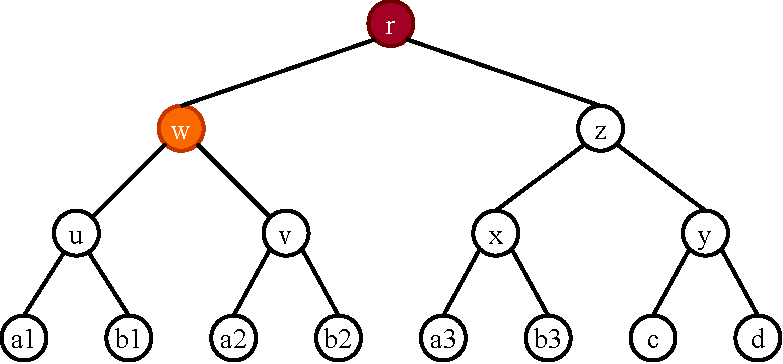
\includegraphics[width=\linewidth]{consistency_score}
  	\caption[Duplication consistency score]{\textbf{Duplication consistency score for node $w$}\\
  	The set of species of left child $u$ is $L = \{A, B\}$ and the set of species of right child $v$ is $R = \{A, B\}$. The duplication consistency score is computed as: $dcs(w) = (L \cup R) \mid (L \cap R) = 2 / 2 = 1$.
  	\\
  	\textbf{Duplication consistency score for node $r$}\\
  	The set of species of left child $w$ is $L = \{A, B\}$ and the set of species of right child $z$ is $R = \{A, B, C, D\}$. The duplication consistency score is computed as: $dcs(r) = (L \cup R) \mid (L \cap R) = 2 / 4 = 0.5$.}
\end{figure}

The real fungi dataset consists of multiple sequence alignment for each gene family of the presented 5351 gene families. To obtain unrooted gene trees from the alignments, we run a RAxML program on each alignment with GTRGAMMA model. We run our software on the acquired unrooted gene trees with tolerance set to $1.0$ and step set to $0.01$ to infer the smallest possible number of duplications and gene losses. To compare, Notung and Treerecs on the acquired gene trees as well (Tab. \ref{real_dataset}). We do not run TreeFix on the real dataset as TreeFix takes only rooted gene trees.

All compared software infer the same number of duplications. The least number of founded gene losses has Treerecs. Our software and Notung infer the same number of gene losses which is higher by $9525$ gene losses from the Treerecs. The duplication consistency score is also highest with Treerecs, which is understandable since it has the smallest number of gene losses. Notung has the duplication consistency score worse by $0.000012$ from the Treerecs. Even though we have the same number of duplications and gene losses with Notung, our duplication consistency score is smaller by $0.000014$ from Notung caused by multiple reconciliation solution, where some of them have duplications with worse duplication consistency score than Notung. The best average running time of computing the reconciliation for each gene tree has Treerecs. Our average running time is worse by $75.22\%$ from Treerecs and better by $20.51\%$ from Notung.

\begin{table}[ht!]
\caption{Results of phylogenetic software on real dataset}
\centering
\begin{threeparttable}
\begin{tabular}{| m{0.25\textwidth} | >{\centering\arraybackslash}m{0.15\textwidth} | >{\centering\arraybackslash}m{0.15\textwidth} | >{\centering\arraybackslash}m{0.15\textwidth} | >{\centering\arraybackslash}m{0.15\textwidth} |}
   \hline
     \textbf{Software\textsuperscript{a}} &
     \textbf{Dup\textsuperscript{b}} &
     \textbf{Loss\textsuperscript{c}} &
     \textbf{DCS\textsuperscript{d}} &
     \textbf{Runtime\textsuperscript{e}}\\
    \hline
    Our & 20534 & 67521 & 0.106953 & 0.679773\\
    Notung & 20534 & 67521 & 0.106967 & 0.855182\\
    Treerecs & 20534 & 57996 & 0.106979 & 0.168448\\
    \hline
    \end{tabular}
  \begin{tablenotes}
                 \footnotesize
                 \item[a] Phylogenetic software with \emph{"t"} as tolerance setting.
                 \item[b] Number of inferred duplications.
                 \item[c] Number of inferred gene losses.
                 \item[d] Average duplication consistency score for each gene tree.
                 \item[e] Average runtime of computing the reconciliation for each gene tree in seconds.
             \end{tablenotes}
         \end{threeparttable}
  \label{real_dataset}
\end{table}




